\chapter{Dispersion and Wave Packets}\label{ch:b2:dispersion-wave-packets}

Drop a stone in a pond and watch the ring of ripples: new crests are
born at its inner edge, run outward through the ring, and die at its
outer edge --- the ring as a whole moves slower than the crests in it.
Sit on a beach after a distant storm and the long, slow swell arrives
a day before the short chop: the sea sorts waves by wavelength. The
first transatlantic telegraph cable, in 1858, turned crisp dots and
dashes into a smear that took minutes to read. In all three cases the
speed of a wave depends on its frequency: the medium is
\emph{dispersive}. This chapter introduces the \omterm{def:b2:dispersion-wave-packets:relation}{dispersion relation}, the
\omterm{def:b2:dispersion-wave-packets:complex}{complex wavenumber} that carries both propagation and absorption, the
\omterm{prop:b2:dispersion-wave-packets:group}{group velocity} at which a packet --- and its energy, and its
information --- actually travels, and the line along which telegraphy,
television and the internet have travelled: the \omterm{prop:b2:dispersion-wave-packets:coax}{coaxial cable}.

\section{The dispersion relation}

\begin{definition}[Dispersion relation; phase velocity]\label{def:b2:dispersion-wave-packets:relation}
\index{dispersion relation}\index{phase velocity}\index{dispersive medium}
A linear, homogeneous, time-invariant medium admits the plane
monochromatic waves $\underline s = A\,\eu^{\iu(\omega t - kx)}$ (complex
notation; the physical signal is the real part) provided $\omega$ and $k$
satisfy the \emph{dispersion relation} of the medium, $\mathcal D(\omega, k)
= 0$, solved as $k(\omega)$ or $\omega(k)$. For real $k$ the wave travels
without deforming at the \emph{phase velocity}
\[
v_\varphi = \frac\omega k .
\]
The medium is \emph{non-dispersive} when $v_\varphi$ does not depend on
$\omega$ (then $\omega = ck$ and every signal propagates undeformed --- the
\omterm{thm:b2:waves-on-strings:equation}{d'Alembert equation}) and \emph{dispersive} otherwise.
\end{definition}

\begin{proof}
Inserting $\eu^{\iu(\omega t - kx)}$ into a linear equation with constant
coefficients turns each $\partial_t$ into $\iu\omega$ and each $\partial_x$ into
$-\iu k$, leaving an algebraic relation. The string, the sound wave and
the rod gave $\omega^2 = c^2k^2$.
\end{proof}

\begin{example}[Dispersive and non-dispersive]\label{ex:b2:dispersion-wave-packets:examples}
\index{Klein--Gordon equation}\index{deep-water waves}
(i) A string on an elastic bed (restoring force $-Ky$ per unit length,
or a chain of pendulums), $\mu\partial_t^2y = T\partial_x^2y - Ky$: $\omega^2 = \omega_c^2
+ c^2k^2$ with $\omega_c = \sqrt{K/\mu}$ --- the \emph{Klein--Gordon}
relation, the same as a plasma's and a waveguide's
(\cref{ch:b2:waves-in-media,ch:b2:guided-waves}): $v_\varphi = c/\sqrt{1 -
\omega_c^2/\omega^2} > c$, and no real $k$ below the \emph{cut-off} $\omega_c$.
(ii) Deep-water gravity waves: $\omega^2 = gk$ (admitted), $v_\varphi =
\sqrt{g/k} = \sqrt{g\lambda/2\pi}$: long waves are faster --- \qty{12.5}{m/s} for
\qty{100}{m}, \qty{40}{m/s} for \qty{1}{km}. (iii) The \omterm{prop:b2:waves-on-strings:chain}{chain of atoms}, $\omega =
2\omega_0|\sin(ka/2)|$ (\cref{ch:b2:waves-on-strings}). (iv) Light in glass,
$k = n(\omega)\omega/c$, which is why a prism spreads a spectrum.
\end{example}

\begin{omfigure}
\begin{tikzpicture}
\begin{axis}[omaxis, axis x line=bottom, axis y line=left, width=6.2cm, height=4.6cm,
    xlabel={$k$}, ylabel={$\omega$}, xmin=0, xmax=3, ymin=0, ymax=3.3, xtick=\empty, ytick={1}, yticklabels={$\omega_c$}, samples=80,
    xlabel style={at={(axis description cs:1.0,0.0)}, anchor=west},
    ylabel style={at={(axis description cs:0.0,1.0)}, anchor=south},
    legend style={font=\scriptsize, at={(0.03,0.97)}, anchor=north west, draw=none, fill=none}]
  \addplot[omDef, thick, domain=0:3] {x};
  \addplot[omThm, thick, domain=0:3] {sqrt(1+x*x)};
  \addplot[omProp, thick, domain=0:3] {1.6*sqrt(x)};
  \legend{$\omega = ck$, $\omega^2 = \omega_c^2 + c^2k^2$, $\omega^2 = gk$}
\end{axis}
\end{tikzpicture}
\hfill
\begin{tikzpicture}
\begin{axis}[omaxis, axis x line=bottom, axis y line=left, width=6.2cm, height=4.6cm,
    xlabel={$\omega/\omega_c$}, ylabel={$v/c$}, xmin=0, xmax=4, ymin=0, ymax=2.6, xtick={1,2,3}, ytick={1}, samples=100,
    xlabel style={at={(axis description cs:0.5,-0.12)}, anchor=north},
    ylabel style={at={(axis description cs:-0.1,0.5)}, rotate=90, anchor=south},
    legend style={font=\scriptsize, at={(0.97,0.95)}, anchor=north east, draw=none, fill=none}]
  \addplot[omThm, thick, domain=1.08:4] {1/sqrt(1-1/(x*x))};
  \addplot[omDef, thick, domain=1.0:4] {sqrt(1-1/(x*x))};
  \addplot[black, dashed, domain=0:4] {1};
  \legend{$v_\varphi$, $v_g$}
  \node[font=\scriptsize, anchor=west, align=left] at (axis cs:0.05,1.9) {no\\propagation};
\end{axis}
\end{tikzpicture}

{\small Left: three \omterm{def:b2:dispersion-wave-packets:relation}{dispersion relations} --- a straight line for a
non-dispersive medium, the Klein--Gordon hyperbola with its cut-off,
the parabola of \omterm{ex:b2:dispersion-wave-packets:examples}{deep-water waves}. Right: for the Klein--Gordon
relation the \omterm{def:b2:dispersion-wave-packets:relation}{phase velocity} exceeds $c$ and the \omterm{prop:b2:dispersion-wave-packets:group}{group velocity} stays
below it, with $v_\varphi v_g = c^2$.}
\end{omfigure}

\begin{definition}[Complex wavenumber: propagation and attenuation]\label{def:b2:dispersion-wave-packets:complex}
\index{complex wavenumber}\index{attenuation}\index{evanescent wave}\index{skin depth}
When the \omterm{def:b2:dispersion-wave-packets:relation}{dispersion relation} gives, for real $\omega$, a complex
$\underline k = k' - \iu k''$, the wave is
\[
\underline s = A\,\eu^{-k''x}\,\eu^{\iu(\omega t - k'x)} :
\]
it propagates at $v_\varphi = \omega/k'$ and its amplitude decays as
$\eu^{-x/\delta}$ with the \emph{attenuation length} $\delta = 1/k''$ (it must
decay in its direction of propagation: $k'$ and $k''$ of the same sign).
If $\underline k$ is purely imaginary, $\underline k = -\iu\kappa$, the wave is
\emph{evanescent}: $A\,\eu^{-\kappa x}\eu^{\iu\omega t}$, a standing oscillation
whose amplitude dies over the distance $1/\kappa$ without propagating
anything --- the case of the Klein--Gordon medium below its cut-off,
$\kappa = \sqrt{\omega_c^2 - \omega^2}/c$, and of a metal at optical frequencies.
\end{definition}

\begin{example}[A damped string]\label{ex:b2:dispersion-wave-packets:damped}
A string in a viscous fluid, $\mu\partial_t^2y + \alpha\partial_ty = T\partial_x^2y$:
$\underline k^2 = (\omega^2 - \iu\alpha\omega/\mu)/c^2$. For weak damping ($\alpha \ll \mu
\omega$), $\underline k \approx \dfrac\omega c\Bigl(1 - \iu\dfrac{\alpha}{2\mu\omega}\Bigr)$: the wave
keeps its speed and loses amplitude over $\delta = 2\mu c/\alpha = 2Z/\alpha$,
independent of frequency --- a \emph{dissipative}, non-dispersive loss,
\qty{8.7}{dB} per length $\delta$.
\end{example}

\section{Wave packets and group velocity}

\begin{proposition}[Beats; group velocity]\label{prop:b2:dispersion-wave-packets:group}
\index{group velocity}\index{wave packet}\index{beats}
Two waves of equal amplitude and neighbouring frequencies $\omega \pm
\delta\omega$, wavenumbers $k \pm \delta k$, superpose into
\[
s = 2A\cos(\delta\omega\,t - \delta k\,x)\cos(\omega t - kx) :
\]
a carrier at $(\omega, k)$ moving at $v_\varphi = \omega/k$, modulated by a slow
envelope moving at $\delta\omega/\delta k$. A \emph{\omterm{prop:b2:dispersion-wave-packets:group}{wave packet}} --- a
superposition of monochromatic waves with wavenumbers in a narrow band
around $k_0$ --- travels, as a whole, at the \emph{\omterm{prop:b2:dispersion-wave-packets:group}{group velocity}}
\[
v_g = \frac{\dd\omega}{\dd k}\Bigr|_{k_0} ,
\]
which is the velocity of its energy and of the information it carries.
In a non-dispersive medium $v_g = v_\varphi = c$; otherwise the packet
deforms as it goes (it \emph{spreads}), the faster the larger
$\dd^2\omega/\dd k^2$ and the narrower its spectrum's complement, its
spatial width.
\end{proposition}

\begin{proof}
The sum-to-product formula gives the beats. For a packet, write $s =
\int a(k)\eu^{\iu(\omega(k)t - kx)}\dd k$ (a Fourier superposition --- the
Fourier integral is studied in the Year 3 mathematics volume; here only
its interpretation as a continuous sum of sinusoids is used), with
$a(k)$ peaked at $k_0$. Expand $\omega(k) \approx \omega_0 + v_g(k - k_0)$: then
$s \approx \eu^{\iu(\omega_0t - k_0x)}\int a(k)\eu^{\iu(k - k_0)(v_gt - x)}\dd k$, a
carrier times an envelope that is a function of $x - v_gt$ only --- the
envelope moves at $v_g$. The next term, $\tfrac12\omega''(k_0)(k - k_0)^2t$,
dephases the components in time and spreads the envelope. The energy
of a packet is located where its envelope is; so is any signal.
\end{proof}

\begin{omfigure}
\begin{tikzpicture}
\begin{axis}[omaxis, axis x line=middle, axis y line=none, width=13.6cm, height=4.0cm,
    xmin=0, xmax=60, ymin=-3.1, ymax=3.3, xtick=\empty, samples=600, xlabel={$x$}, clip=false,
    xlabel style={at={(axis description cs:1.0,0.5)}, anchor=west}]
  \addplot[omDef, thick, domain=0:60] {2*cos(deg(0.12*x))*cos(deg(2.2*x))};
  \addplot[omThm, thick, domain=0:60] {2*cos(deg(0.12*x))};
  \addplot[omThm, thick, domain=0:60] {-2*cos(deg(0.12*x))};
  \draw[omThm, very thick, ->] (axis cs:9,2.6) -- (axis cs:15,2.6) node[above, font=\scriptsize, pos=0.5] {$v_g$};
  \draw[omDef, very thick, ->] (axis cs:38,-2.6) -- (axis cs:48,-2.6) node[below, font=\scriptsize, pos=0.5] {$v_\varphi$};
\end{axis}
\end{tikzpicture}

{\small Beats: two neighbouring frequencies produce a fast carrier
(moving at the \omterm{def:b2:dispersion-wave-packets:relation}{phase velocity}) under a slow envelope (moving at the
\omterm{prop:b2:dispersion-wave-packets:group}{group velocity}); in a \omterm{def:b2:dispersion-wave-packets:relation}{dispersive medium} the two speeds differ and the
crests slide through the envelope.}
\end{omfigure}

\begin{example}[Deep water: the crests outrun the group]\label{ex:b2:dispersion-wave-packets:deepwater}
$\omega = \sqrt{gk}$: $v_g = \tfrac12\sqrt{g/k} = \tfrac12v_\varphi$. A group of
swell moves at half the speed of its crests: watching a wave train,
you see crests appear at the back of the group, travel through it and
vanish at the front --- exactly the pond's ring. A storm \qty{3000}{km}
away sends its \qty{15}{s} swell ($\lambda = gT^2/2\pi = \qty{350}{m}$, $v_g =
gT/4\pi = \qty{11.7}{m/s}$) in three days, its \qty{8}{s} waves ($v_g =
\qty{6.2}{m/s}$) in five and a half: from the arrival times of the
different periods, oceanographers locate the storm.
\end{example}

\begin{omfigure}
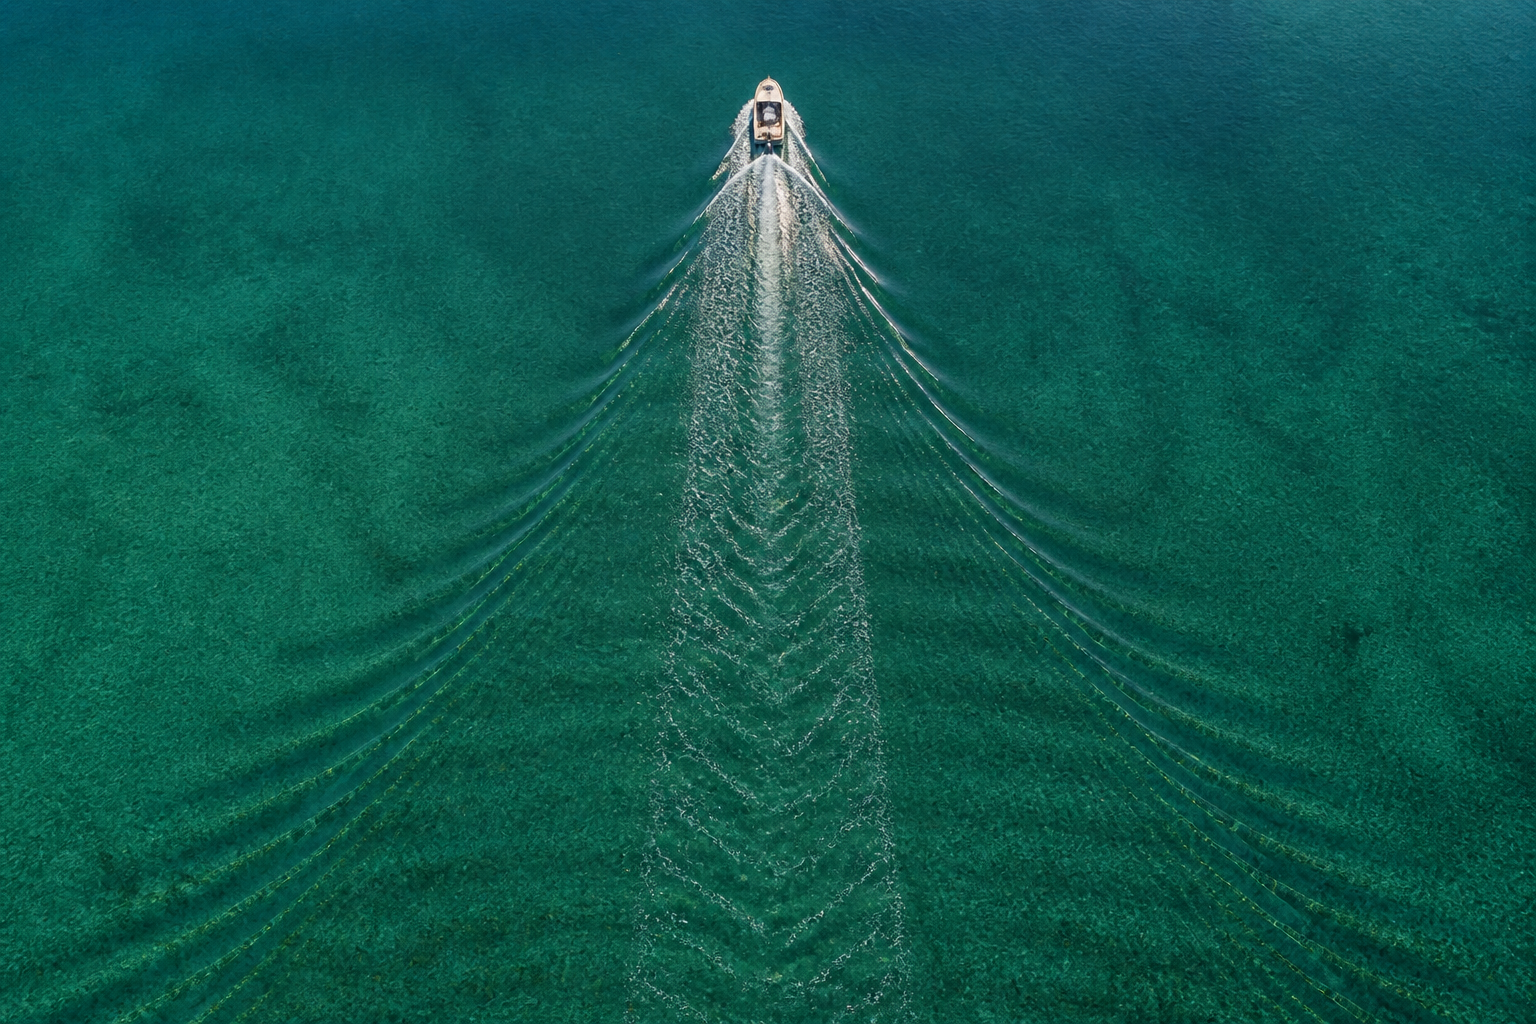
\includegraphics[width=0.56\linewidth]{images/book4/ai/b4-08-boat-wake-aerial.png}

{\small The wake of a motorboat on a calm lake: the feathered pattern stays inside a wedge of fixed angle because the energy of each water wave travels at half the speed of its crests --- dispersion made visible.}
\end{omfigure}


\begin{example}[Klein--Gordon: faster than light, and not]\label{ex:b2:dispersion-wave-packets:superluminal}
For $\omega^2 = \omega_c^2 + c^2k^2$: $v_\varphi = \omega/k$ and $v_g = c^2k/\omega$, so
$v_\varphi v_g = c^2$: the \omterm{def:b2:dispersion-wave-packets:relation}{phase velocity} exceeds $c$ (in the ionosphere, a
\qty{10}{MHz} wave's crests move faster than light) but the \omterm{prop:b2:dispersion-wave-packets:group}{group
velocity}, which carries the signal, stays below it. A \omterm{def:b2:dispersion-wave-packets:relation}{phase velocity}
transports no energy and no information --- the crests are like the
spot of a lighthouse beam sweeping a distant cloud.
\end{example}

\begin{remark}[Spreading]\label{rem:b2:dispersion-wave-packets:spreading}
A packet of spatial width $\Delta x$ contains wavenumbers over $\Delta k \sim
1/\Delta x$ (the Fourier reciprocity, admitted); its components' group
velocities differ by $\Delta v_g \approx |\omega''|\Delta k$, so after a time $t$ it
has spread by $|\omega''|\Delta k\,t$: it doubles its width after $t_{\text{sp}}
\sim \Delta x^2/|\omega''|$. A packet of ten \omterm{ex:b2:dispersion-wave-packets:examples}{deep-water waves} of \qty{100}{m}
($\Delta x \approx \qty{1}{km}$, $\omega'' = -\tfrac14\sqrt{g/k^3} = \qty{-50}{m^2/s}$)
doubles in about six hours; a light pulse of \qty{1}{ns} in an
optical fibre spreads by tens of picoseconds per kilometre --- the
limit of the bit rate of long links. The quantum \omterm{prop:b2:dispersion-wave-packets:group}{wave packet} of
\cref{ch:b2:schrodinger-wave-functions} spreads for the same reason.
\end{remark}

\section{The coaxial cable}

\begin{proposition}[Telegrapher's equations; lossless line]\label{prop:b2:dispersion-wave-packets:coax}
\index{coaxial cable}\index{telegrapher's equations}\index{characteristic impedance}\index{transmission line}
A \omterm{prop:b2:dispersion-wave-packets:coax}{coaxial cable} (or any two-conductor line) has, per unit length, an
inductance $\Lambda$ and a capacitance $\Gamma$. The voltage $v(x, t)$ between
the conductors and the current $i(x, t)$ in the inner one obey the
\emph{\omterm{prop:b2:dispersion-wave-packets:coax}{telegrapher's equations}}
\[
\frac{\partial v}{\partial x} = -\Lambda\frac{\partial i}{\partial t} , \qquad
\frac{\partial i}{\partial x} = -\Gamma\frac{\partial v}{\partial t} ,
\]
hence the \omterm{thm:b2:waves-on-strings:equation}{d'Alembert equation} for $v$ and $i$ with
\[
c = \frac1{\sqrt{\Lambda\Gamma}} , \qquad
v = Z_c\,i \ \text{for a wave toward } +x, \quad Z_c = \sqrt{\frac\Lambda\Gamma} ,
\]
$Z_c$ being the \emph{\omterm{prop:b2:dispersion-wave-packets:coax}{characteristic impedance}} of the line. For a
\omterm{prop:b2:dispersion-wave-packets:coax}{coaxial cable} of radii $a < b$ filled with a dielectric of relative
permittivity $\varepsilon_r$, $\Lambda = \dfrac{\mu_0}{2\pi}\ln\dfrac ba$, $\Gamma =
\dfrac{2\pi\varepsilon_0\varepsilon_r}{\ln(b/a)}$, so $c = c_0/\sqrt{\varepsilon_r}$ (about
\qty{2e8}{m/s}, two thirds of the speed of light) and $Z_c = \dfrac{60\,\Omega}
{\sqrt{\varepsilon_r}}\ln\dfrac ba$: \qty{50}{\ohm} or \qty{75}{\ohm} for the usual cables.
\end{proposition}

\begin{proof}
Model the slice $[x, x + \dd x]$ as a series inductance $\Lambda\dd x$ and a
shunt capacitance $\Gamma\dd x$: the voltage drop along the slice is
$\Lambda\dd x\,\partial_ti$, and the current lost into the capacitance is $\Gamma\dd x
\,\partial_tv$. Cross-differentiate. For $v = f(x - ct)$, the first equation
gives $i = f(x - ct)/\Lambda c = v/\sqrt{\Lambda/\Gamma}$. The values of $\Lambda$ and
$\Gamma$ are those of the cylindrical capacitor and of the coaxial
inductor computed in the Year 1 volume.
\end{proof}

\begin{omfigure}
\begin{tikzpicture}[font=\small]
  \begin{scope}
    \draw (0,0) to[L, l=$\Lambda\,\dd x$] (2.2,0) to[C, l=$\Gamma\,\dd x$] (2.2,-1.6);
    \draw (0,-1.6) -- (2.2,-1.6);
    \draw (2.2,0) -- (3.8,0); \draw (2.2,-1.6) -- (3.8,-1.6);
    \draw[->] (0.1,0.35) -- (0.7,0.35); \node[font=\footnotesize] at (0.4,0.6) {$i(x)$};
    \draw[->] (2.9,0.35) -- (3.5,0.35); \node[font=\footnotesize] at (3.2,0.6) {$i(x+\dd x)$};
    \node[font=\footnotesize] at (-0.3,-0.8) {$v(x)$}; \node[font=\footnotesize] at (4.6,-0.8) {$v(x+\dd x)$};
    \draw (-0.6,-0.2) -- (-0.6,-1.4); \draw[->] (-0.6,-1.4) -- (-0.6,-0.3);
    \node[font=\footnotesize] at (1.6,-2.3) {one slice of the line};
  \end{scope}
  \begin{scope}[xshift=8.4cm, yshift=-0.8cm]
    \draw[thick, fill=omExo!30] (0,0) circle (1.3);
    \draw[thick, fill=omDef!15] (0,0) circle (1.05);
    \draw[thick, fill=omThm!40] (0,0) circle (0.3);
    \draw[<->] (0,0) -- (30:0.3) node[pos=1.6, font=\footnotesize] {$a$};
    \draw[<->] (0,0) -- (-50:1.05) node[pos=0.6, right, font=\footnotesize] {$b$};
    \node[font=\footnotesize] at (0,1.65) {$\varepsilon_r$ dielectric, braid, core};
    \node[font=\footnotesize] at (0,-1.75) {$Z_c = \dfrac{60\,\Omega}{\sqrt{\varepsilon_r}}\ln\dfrac ba$};
  \end{scope}
\end{tikzpicture}

{\small Left: the equivalent circuit of a slice $\dd x$ of a lossless
line --- series inductance, shunt capacitance --- from which the
\omterm{prop:b2:dispersion-wave-packets:coax}{telegrapher's equations} follow. Right: a \omterm{prop:b2:dispersion-wave-packets:coax}{coaxial cable} in section; its
$\Lambda$ and $\Gamma$ depend only on the ratio of radii and on the
dielectric.}
\end{omfigure}

\begin{omfigure}
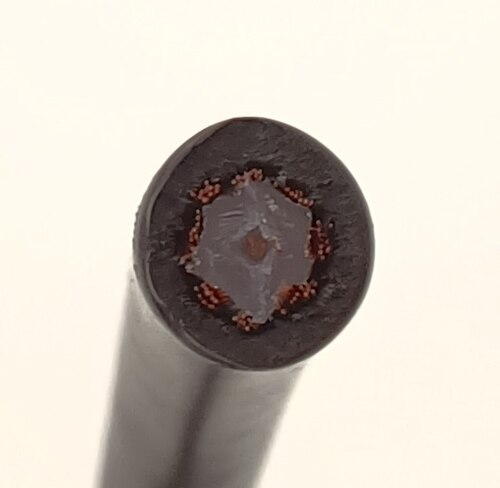
\includegraphics[width=0.46\linewidth]{images/book3/coaxial-cable.jpg}

{\small A \omterm{prop:b2:dispersion-wave-packets:coax}{coaxial cable}: inner core, dielectric, braided outer conductor --- a \omterm{prop:b2:dispersion-wave-packets:coax}{transmission line} whose inductance and capacitance per metre set its speed and its \omterm{prop:b2:dispersion-wave-packets:coax}{characteristic impedance}.}
\end{omfigure}

\begin{proposition}[Lossy line; the distortionless condition]\label{prop:b2:dispersion-wave-packets:lossy}
\index{Heaviside condition}\index{Kelvin's law of squares}
With a series resistance $R$ and a shunt conductance $G$ per unit
length, the equations become $\partial_xv = -\Lambda\partial_ti - Ri$, $\partial_xi =
-\Gamma\partial_tv - Gv$, and the \omterm{def:b2:dispersion-wave-packets:relation}{dispersion relation} $\underline k^2 = (\Lambda\omega -
\iu R)(\Gamma\omega - \iu G)$: the line is dispersive and attenuating. Two
limits: (i) $R/\Lambda = G/\Gamma$ (Heaviside's condition, reached by adding
inductance): $\underline k = \omega\sqrt{\Lambda\Gamma} - \iu\sqrt{RG}$, every frequency
travels at the same speed with the same \omterm{def:b2:dispersion-wave-packets:complex}{attenuation} --- the line
\emph{attenuates} but does not \emph{distort}. (ii) $\Lambda \approx 0$, $G \approx 0$
(the first submarine cables): $\partial_x^2v = R\Gamma\,\partial_tv$, a
\emph{diffusion} equation --- a pulse does not propagate but smears,
reaching a distance $L$ after a time $\sim R\Gamma L^2$ (Kelvin's law of
squares), a hundred times longer for a cable ten times longer.
\end{proposition}

\begin{proof}
Insert $\eu^{\iu(\omega t - kx)}$: $-\iu kv = -(\iu\omega\Lambda + R)i$, $-\iu ki = -(\iu
\omega\Gamma + G)v$; multiply. Under Heaviside's condition the product is a
perfect square. The diffusion limit drops the $\iu\omega\Lambda$ and $G$ terms.
\end{proof}

\begin{example}[Three cables]\label{ex:b2:dispersion-wave-packets:cables}
The 1858 transatlantic cable: a single copper wire in gutta-percha,
$R \approx \qty{3}{\ohm/km}$, $\Gamma \approx \qty{0.3}{\micro F/km}$, $L = \qty{3000}{km}$:
$R\Gamma = \qty{9e-10}{s/m^2}$ and $R\Gamma L^2 \approx \qty{8}{s}$ per dot: a word a
minute, and the operators' attempts to force the signal
with \qty{2}{kV} destroyed the insulation within weeks. A telephone line
loaded with coils every \qty{2}{km} to satisfy Heaviside's condition
(1900): clear speech over hundreds of kilometres. A modern \qty{50}{\ohm}
\omterm{prop:b2:dispersion-wave-packets:coax}{coaxial cable}: $c = \qty{2e8}{m/s}$, $\Lambda = \qty{0.25}{\micro H/m}$, $\Gamma =
\qty{100}{pF/m}$, and an \omterm{def:b2:dispersion-wave-packets:complex}{attenuation}, due to the skin effect in the
conductors (\cref{ch:b2:waves-in-media}), growing as $\sqrt f$: a few
\omterm{def:b2:sound-waves:decibel}{decibels} per hundred metres at \qty{100}{MHz}.
\end{example}

\begin{method}[Reading a dispersion relation]\label{met:b2:dispersion-wave-packets:method}
(1) Write the \omterm{thm:b2:waves-on-strings:equation}{wave equation} of the medium in complex notation and
solve for $\underline k(\omega)$. (2) Real $k$: compute $v_\varphi = \omega/k$ and
$v_g = \dd\omega/\dd k$ (or $1/(\dd k/\dd\omega)$); compare: dispersive or not,
normal ($v_g < v_\varphi$) or anomalous. (3) Complex $k$: split into
propagation ($k'$) and \omterm{def:b2:dispersion-wave-packets:complex}{attenuation} ($k''$, length $1/k''$); purely
imaginary means evanescent, no transport. (4) A cut-off frequency
separates a propagating band from an evanescent one. (5) For a signal,
reason on the envelope at $v_g$, never on the crests.
\end{method}

\section{Exercises}

\begin{exercise}[$\star$]\label{exo:b2:dispersion-wave-packets:1}
\omterm{ex:b2:dispersion-wave-packets:examples}{Deep-water waves}, $\omega^2 = gk$. (a) \omterm{def:b2:dispersion-wave-packets:relation}{Phase velocity}, \omterm{prop:b2:dispersion-wave-packets:group}{group velocity} and
period of a \qty{100}{m} swell. (b) A swell of period \qty{14}{s}:
wavelength, $v_\varphi$, $v_g$; time for its energy to cross \qty{5000}{km}.
(c) Why does the chop of a \qty{2}{s} period not get there at all?
\end{exercise}

\begin{exercise}[$\star$]\label{exo:b2:dispersion-wave-packets:2}
A medium obeys $\omega^2 = \omega_c^2 + c^2k^2$ with $\omega_c = 2\pi \times \qty{1e7}{rad/s}$
and $c = \qty{3e8}{m/s}$. For $f = \qty{20}{MHz}$: $k$, $v_\varphi$, $v_g$, and
their product. For $f = \qty{5}{MHz}$: $\kappa$ and the penetration depth.
\end{exercise}

\begin{exercise}[$\star$]\label{exo:b2:dispersion-wave-packets:3}
Two tuning forks at \qty{440}{Hz} and \qty{444}{Hz}: beat frequency, and
the period of the loudness variations. Two water waves of wavelengths
\qty{100}{m} and \qty{110}{m}: frequencies, wavelength and speed of the
envelope; compare with $v_g$ at \qty{105}{m}.
\end{exercise}

\begin{exercise}[$\star$]\label{exo:b2:dispersion-wave-packets:4}
A \omterm{prop:b2:dispersion-wave-packets:coax}{coaxial cable}: inner conductor \qty{0.9}{mm} in diameter, outer
\qty{3.0}{mm}, polyethylene ($\varepsilon_r = 2.3$). $\Lambda$, $\Gamma$, wave speed,
\omterm{prop:b2:dispersion-wave-packets:coax}{characteristic impedance}, delay per metre; length of cable equivalent
to a \qty{10}{ns} delay. Same cable with air instead of polyethylene.
\end{exercise}

\begin{exercise}[$\star\star$]\label{exo:b2:dispersion-wave-packets:5}
\emph{The stiff string.} A real piano string obeys $\mu\partial_t^2y = T\partial_x^2y
- EI\,\partial_x^4y$ ($EI$ the bending stiffness). (a) \omterm{def:b2:dispersion-wave-packets:relation}{Dispersion relation},
phase and group velocities. (b) For the A$_4$ string of
\cref{ch:b2:waves-on-strings} ($T = \qty{685}{N}$, $\mu = \qty{6.1}{g/m}$, $EI =
\qty{9.8e-3}{N.m^2}$), relative increase of $v_\varphi$ for the eighth
harmonic ($k = 8\pi/L$, $L = \qty{0.38}{m}$); check against the inharmonicity
found there. (c) Is the dispersion normal or anomalous? What does a
sharp pluck look like after a few round trips?
\end{exercise}

\begin{exercise}[$\star\star$]\label{exo:b2:dispersion-wave-packets:6}
\emph{Damped string.} $\mu\partial_t^2y + \alpha\partial_ty = T\partial_x^2y$. (a) Derive
the \omterm{def:b2:dispersion-wave-packets:relation}{dispersion relation}. (b) For $\alpha \ll \mu\omega$, show $k' \approx \omega/c$ and
$k'' \approx \alpha/2Z$; \omterm{def:b2:dispersion-wave-packets:complex}{attenuation} in \omterm{def:b2:sound-waves:decibel}{decibels} per metre. (c) Numbers: $\mu =
\qty{5}{g/m}$, $T = \qty{50}{N}$, $\alpha = \qty{0.02}{kg.m^{-1}.s^{-1}}$, $f =
\qty{100}{Hz}$: check the approximation and give $\delta$. (d) Is the damped
string dispersive? In which regime of $\alpha$ would it become so?
\end{exercise}

\begin{exercise}[$\star\star$]\label{exo:b2:dispersion-wave-packets:7}
\emph{Ripples.} Short water waves are ruled by \omterm{rem:b2:viscous-flows:capillarity}{surface tension}: $\omega^2 =
\gamma k^3/\rho$ ($\gamma = \qty{0.072}{N/m}$); the full relation is $\omega^2 = gk +
\gamma k^3/\rho$. (a) $v_\varphi$ and $v_g$ for pure capillary waves; which is
larger? (b) Show that the \omterm{def:b2:dispersion-wave-packets:relation}{phase velocity} of the full relation is
minimal at $\lambda_m = 2\pi\sqrt{\gamma/\rho g}$ and compute $\lambda_m$ and $v_{\min}$.
(c) A boat slower than $v_{\min}$ makes no wake: why? (d) Raindrops on a
pond make rings whose crests lag behind the ring: in which regime?
\end{exercise}

\begin{exercise}[$\star\star$]\label{exo:b2:dispersion-wave-packets:8}
\emph{Spreading.} A packet of initial width $\Delta x_0$ doubles its width
after $t_{\text{sp}} \approx \Delta x_0^2/|\omega''(k_0)|$. (a) A group of \omterm{ex:b2:dispersion-wave-packets:examples}{deep-water
waves}, $\lambda = \qty{50}{m}$, $\Delta x_0 = \qty{500}{m}$. (b) A pulse of light in
a glass fibre: $\omega'' \approx \qty{-0.16}{m^2/s}$; a \qty{10}{ps} pulse ($\Delta x_0 =
\qty{2}{mm}$): spreading time and the distance travelled meanwhile; the same
for a \qty{1}{ns} pulse. Why do long optical links use longer pulses or
dispersion-compensating fibre?
\end{exercise}

\begin{exercise}[$\star\star$]\label{exo:b2:dispersion-wave-packets:9}
\emph{The submarine cable.} $R = \qty{3}{\ohm/km}$, $\Gamma = \qty{0.3}{\micro F/km}$,
$\Lambda$ and $G$ negligible. (a) Show that $v$ obeys a diffusion equation and
give its diffusivity. (b) \omterm{def:b2:dispersion-wave-packets:relation}{Dispersion relation} $\underline k(\omega)$; \omterm{def:b2:dispersion-wave-packets:relation}{phase
velocity} and \omterm{def:b2:dispersion-wave-packets:complex}{attenuation} length at \qty{1}{Hz} and at \qty{10}{Hz}. (c)
Time for a signal to "arrive" over \qty{3000}{km} ($\sim R\Gamma L^2$); words per
minute. (d) Heaviside's cure: the inductance per kilometre needed for
$R/\Lambda = G/\Gamma$ if $G = \qty{1e-7}{S/km}$; why was it hard to add?
\end{exercise}

\begin{exercise}[$\star\star\star$]\label{exo:b2:dispersion-wave-packets:10}
\emph{Energy travels at the \omterm{prop:b2:dispersion-wave-packets:group}{group velocity}.} String on an elastic bed:
$\mu\partial_t^2y = T\partial_x^2y - Ky$, wave $y = A\cos(\omega t - kx)$ with $\omega^2 =
\omega_c^2 + c^2k^2$. (a) Energy density $e = \tfrac12\mu(\partial_ty)^2 + \tfrac12T
(\partial_xy)^2 + \tfrac12Ky^2$ and flux $\mathcal P = -T\partial_xy\,\partial_ty$: check
$\partial_te + \partial_x\mathcal P = 0$. (b) Time averages $\langle e\rangle$ and
$\langle\mathcal P\rangle$ for the wave. (c) Show that $\langle\mathcal P\rangle/
\langle e\rangle = c^2k/\omega = v_g$, not $v_\varphi$. (d) What happens to the
energy flux below the cut-off?
\end{exercise}

\begin{exercise}[$\star\star\star$]\label{exo:b2:dispersion-wave-packets:11}
\emph{Swell and tsunami.} Water waves of wavelength $\lambda$ on a depth $h$
obey $\omega^2 = gk\tanh kh$ (admitted). (a) Recover the deep-water and the
shallow-water ($kh \ll 1$) limits; speed of shallow-water waves; are
they dispersive? (b) A tsunami of $\lambda = \qty{200}{km}$ on \qty{4}{km} of ocean:
which limit, speed, period; time to cross \qty{8000}{km}. (c) Its
amplitude offshore is \qty{0.5}{m}: energy per unit length of crest
(admit $E = \tfrac12\rho gA^2$ per unit area) for a \qty{1000}{km} front; what
happens when the depth falls to \qty{10}{m}, if the energy flux $Ev_g$ is
conserved (Green's law, $A \propto h^{-1/4}$)? (d) A \qty{100}{m} swell
arriving on a beach: at what depth does it start to feel the bottom,
and why do its crests turn parallel to the shore?
\end{exercise}

\begin{exercise}[$\star\star\star$]\label{exo:b2:dispersion-wave-packets:12}
\emph{A pulse on a line.} A \qty{50}{\ohm} cable of length $\ell = \qty{100}{m}$
($c = \qty{2e8}{m/s}$) is fed at $x = 0$ by a generator of internal
resistance \qty{50}{\ohm} and ended at $x = \ell$ by a load $R_L$. (a) Show
that a wave arriving at the end is reflected with the voltage
coefficient $r = (R_L - Z_c)/(R_L + Z_c)$ (write $v$ and $i$ as incident
plus reflected waves and impose Ohm's law in the load). (b) Values for
$R_L = 50$, $0$, $\infty$, \qty{150}{\ohm}. (c) A \qty{1}{ns} pulse of \qty{1}{V} is
sent: what the oscilloscope at the generator shows, and when, for each
load; why the generator's \qty{50}{\ohm} matter. (d) A fault in a buried
cable returns an echo after \qty{1.8}{\micro s}: where is it? (Time-domain
reflectometry.)
\end{exercise}

\section{Problem: The cable and the sea}

\begin{problem}[{Weekend problem --- dispersion at work: the telegraph
cable that smeared the dots, the swell that announces a storm, the
tsunami that crosses an ocean, and the packet that spreads}]
\label{pb:b2:dispersion-wave-packets:1}

\medskip
\noindent\textbf{Part I --- The telegraph cable.}
The 1866 transatlantic cable: $R = \qty{2.0}{\ohm/km}$, $\Gamma = \qty{0.25}{\micro F/km}$,
$\Lambda = \qty{0.5}{mH/km}$, $G$ negligible, length $L = \qty{3500}{km}$.
\begin{enumerate}
  \item Write the \omterm{prop:b2:dispersion-wave-packets:coax}{telegrapher's equations} with $R$ and derive the
        \omterm{def:b2:dispersion-wave-packets:relation}{dispersion relation} $\underline k^2 = \Gamma\omega(\Lambda\omega - \iu R)$.
  \item At what frequency does $\Lambda\omega$ equal $R$? Conclude that for
        telegraph frequencies (a few hertz) the line is in the
        diffusive regime.
  \item In that regime, $\underline k = \sqrt{-\iu R\Gamma\omega}$: give $k'$ and $k''$
        (recall $\sqrt{-\iu} = (1 - \iu)/\sqrt2$); \omterm{def:b2:dispersion-wave-packets:relation}{phase velocity} and
        \omterm{def:b2:dispersion-wave-packets:complex}{attenuation} length at \qty{1}{Hz}; at \qty{4}{Hz}.
  \item \omterm{def:b2:dispersion-wave-packets:complex}{Attenuation} in \omterm{def:b2:sound-waves:decibel}{decibels} over the whole cable at \qty{1}{Hz} and
        at \qty{4}{Hz}. Which frequency survives? What does that do to a
        sharp dot?
  \item Kelvin's estimate of the transit time, $R\Gamma L^2$; the practical
        rate of the cable in words per minute if a word is about
        $10$ dots and dashes and the dots must not overlap.
  \item Heaviside proposed to raise $\Lambda$: what value makes $\Lambda\omega = R$
        at \qty{4}{Hz}, and what would the speed and \omterm{def:b2:dispersion-wave-packets:complex}{attenuation} then be
        (take $G = 0$, so the condition $R/\Lambda = G/\Gamma$ cannot be met
        exactly --- use the general relation at that frequency)?
  \item A modern optical fibre carries \qty{1e10}{bit/s}: compare with
        question 5, in powers of ten.
\end{enumerate}

\medskip
\noindent\textbf{Part II --- The swell.}
Deep water: $\omega^2 = gk$.
\begin{enumerate}[resume]
  \item Phase and \omterm{prop:b2:dispersion-wave-packets:group}{group velocity} as functions of the period $T$.
  \item A storm \qty{4000}{km} from a coast generates waves of periods
        from \qty{6}{s} to \qty{18}{s}: arrival time of each extreme;
        duration of the swell event.
  \item Show that at a coast at distance $D$ the arriving period obeys
        $1/T = gt/4\pi D$, $t$ counted from the storm: $1/T$ grows
        linearly in time. A buoy records $T = \qty{16}{s}$ one day at noon
        and $T = \qty{12}{s}$ exactly \qty{24}{h} later: distance of the
        storm.
  \item Energy per unit area of a swell of amplitude $A$ is $\tfrac12\rho
        gA^2$; power crossing a line of \qty{1}{m} of crest, for $A =
        \qty{1.5}{m}$, $T = \qty{12}{s}$. (Use the \omterm{prop:b2:dispersion-wave-packets:group}{group velocity} --- why?)
  \item A wave-energy farm of \qty{1}{km} of front with $30\%$ efficiency:
        electrical power; compare with a wind turbine (\qty{3}{MW}).
  \item A boat at \qty{5}{m/s} on deep water leaves a stationary wake
        behind it: which wavelength has a \omterm{def:b2:dispersion-wave-packets:relation}{phase velocity} equal to the
        boat's speed and so follows it? Why does the pattern trail in
        a V, narrower than the crests' own spreading would suggest
        (think of $v_g = v_\varphi/2$)?
  \item Watching one group of swell from a cliff, describe what an
        individual crest does during the time the group passes a
        fixed buoy; how many crests does a group of duration
        \qty{2}{min} contain at $T = \qty{12}{s}$, and how many crest
        "lifetimes" does that represent?
\end{enumerate}

\medskip
\noindent\textbf{Part III --- The tsunami.}
$\omega^2 = gk\tanh kh$; Pacific depth $h = \qty{4.0}{km}$.
\begin{enumerate}[resume]
  \item An earthquake lifts a sea-floor patch of \qty{100}{km} by
        \qty{2}{m}; the wave has $\lambda \approx \qty{200}{km}$: check that it is a
        shallow-water wave and give its speed, period and the time to
        reach a coast \qty{6000}{km} away.
  \item Is it dispersive? Compare with the swell of Part II: does it
        arrive before or after the swell would? Which arrives as a
        single pulse?
  \item Its height offshore is \qty{0.6}{m}: energy per square metre;
        total energy of a \qty{500}{km}-long front spread over one
        wavelength; compare with a \qty{1}{Mt} explosion (\qty{4.2e15}{J}).
  \item Green's law: height when the depth falls to \qty{20}{m} near the
        shore (energy flux $\tfrac12\rho gA^2v_g$ conserved, $v_g = \sqrt{gh}$);
        speed and wavelength there; why the wave then steepens and
        breaks like a wall.
  \item A ship at sea does not notice the tsunami passing: why?
  \item Tide gauges \qty{6000}{km} apart record the wave: what the
        travel time gives, and why the measured speed is slightly
        less than $\sqrt{gh}$ over an ocean of varying depth.
\end{enumerate}

\medskip
\noindent\textbf{Part IV --- The spreading packet.}
\begin{enumerate}[resume]
  \item For deep water, compute $\omega''(k) = \dd^2\omega/\dd k^2$ and its value
        for $\lambda = \qty{100}{m}$.
  \item A packet of \qty{10}{} such waves ($\Delta x_0 \approx \qty{1}{km}$) is
        released: spreading time $\Delta x_0^2/|\omega''|$; distance travelled
        by the packet meanwhile.
  \item Explain in words why a packet with a narrower spectrum
        (longer train) spreads more slowly, and why the tsunami of
        Part III barely spreads at all.
  \item The same estimate for an electron of wavelength \qty{0.1}{nm}
        localized within \qty{1}{nm}, with $\omega = \hbar k^2/2m$ ($\hbar =
        \qty{1.05e-34}{J.s}$, $m = \qty{9.1e-31}{kg}$): spreading time and
        the distance travelled --- the first contact with the quantum
        \omterm{prop:b2:dispersion-wave-packets:group}{wave packet} of \cref{ch:b2:schrodinger-wave-functions}.
  \item Sum up in a table: for the cable, the swell, the tsunami and
        the electron, the \omterm{def:b2:dispersion-wave-packets:relation}{dispersion relation}, $v_\varphi$, $v_g$ and
        whether the medium spreads or merely attenuates.
\end{enumerate}
\end{problem}
